\begin{frame}{Un peu d'histoire}
    \begin{itemize}
        \item mars 2013 : Release par Solomon Hykes (dotcloud)
        \item octobre 2013 : dotcloud devient Docker, Inc
        \item 2014 : passage de Linux containers à libcontainers (Golang)
        \item 2014 : partenariat avec Amazon EC2 et IBM
        \item 2015 : Succès Github (plus de 1100 contributeurs)
        \item 2016 : Windocks, portage du projet à Windows 
        \item 2017 : 13 milliards de téléchargements, + 160\% de mentions sur LinkedIn par rapport à 2016
        \item 2019 : 1917 contributeurs, 43 573 commits
    \end{itemize}
\end{frame}

\begin{frame}{En bref}
    \begin{itemize}
        \item Projet Open Source
        \item Gestionnaire de containers
        \item Peut tourner dans une machine virtuelle
        \item Permet de faire tourner des micro services sur une architecture distribuée
    \end{itemize}
\end{frame}

\begin{frame}{Container et machine virtuelle}
    \begin{block}{Container}
         Un container est un \textbf{package exécutable, léger et autonome} qui contient tout ce qu'il faut pour faire tourner un logiciel et qui est \textbf{indépendant du système d'exploitation}.
    \end{block}
    
    \begin{block}{Machine Virtuelle}
         Une machine virtuelle est une \textbf{émulation de ressources matérielles et logicielles} telles que la mémoire, le processeur, le disque dur, et le système d'exploitation qui permet d'exécuter les programmes dans les mêmes conditions que la machine simulée. Ça permet une grande \textbf{portabilité des logiciels}.
    \end{block}
\end{frame}

\begin{frame}{Containers vs Machine Virtuelle}
    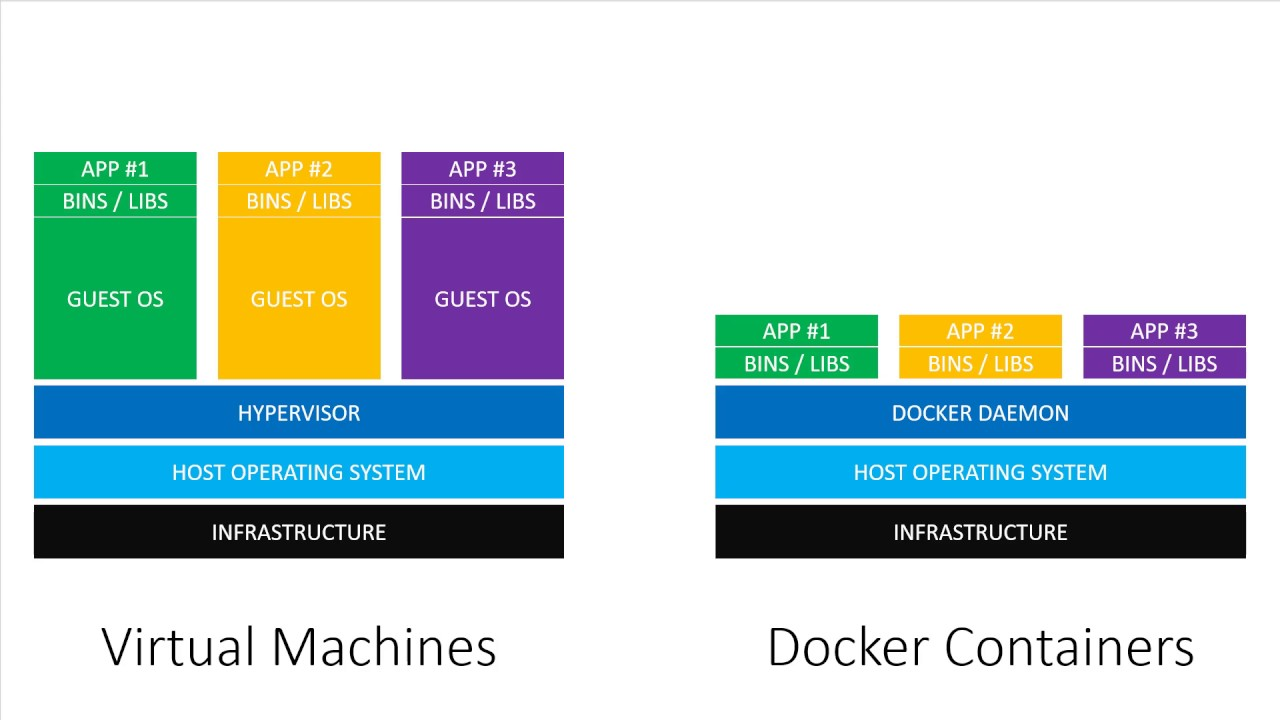
\includegraphics[width=10cm]{img/dockerVSVM.jpg}
\end{frame}

\begin{frame}{Architecture}
    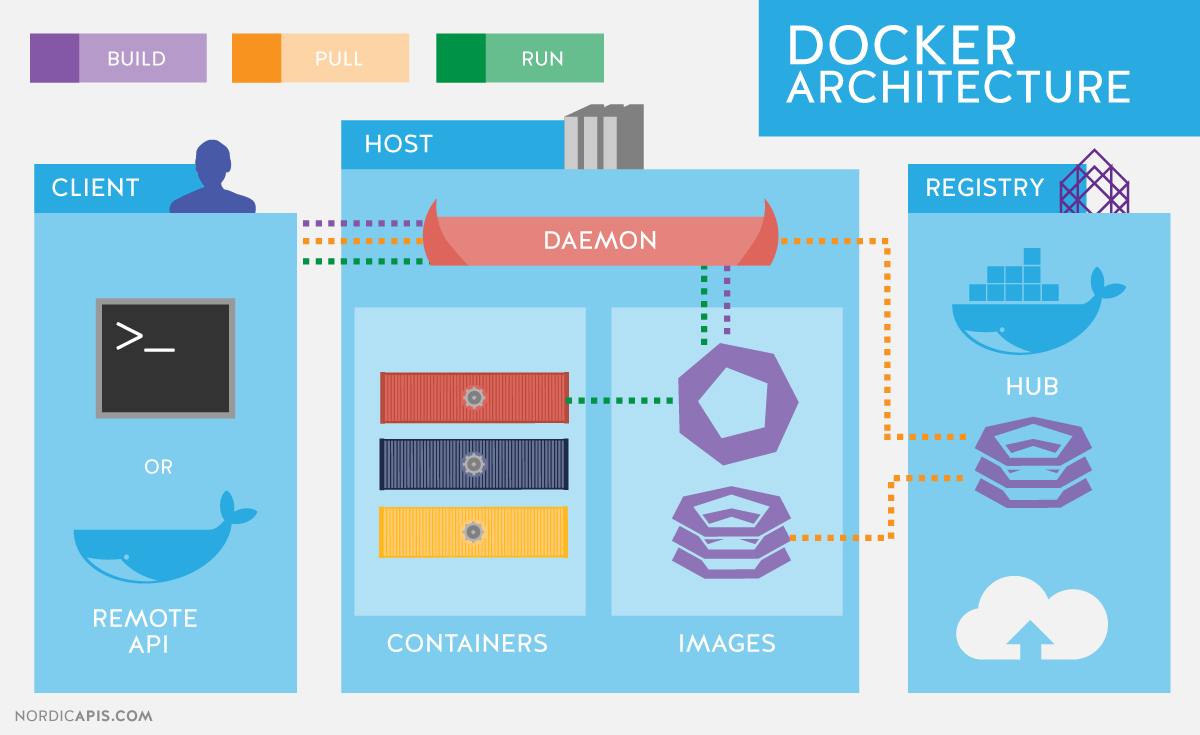
\includegraphics[width=10cm]{img/architecture.png}
\end{frame}

\begin{frame}{Organisation courante}
    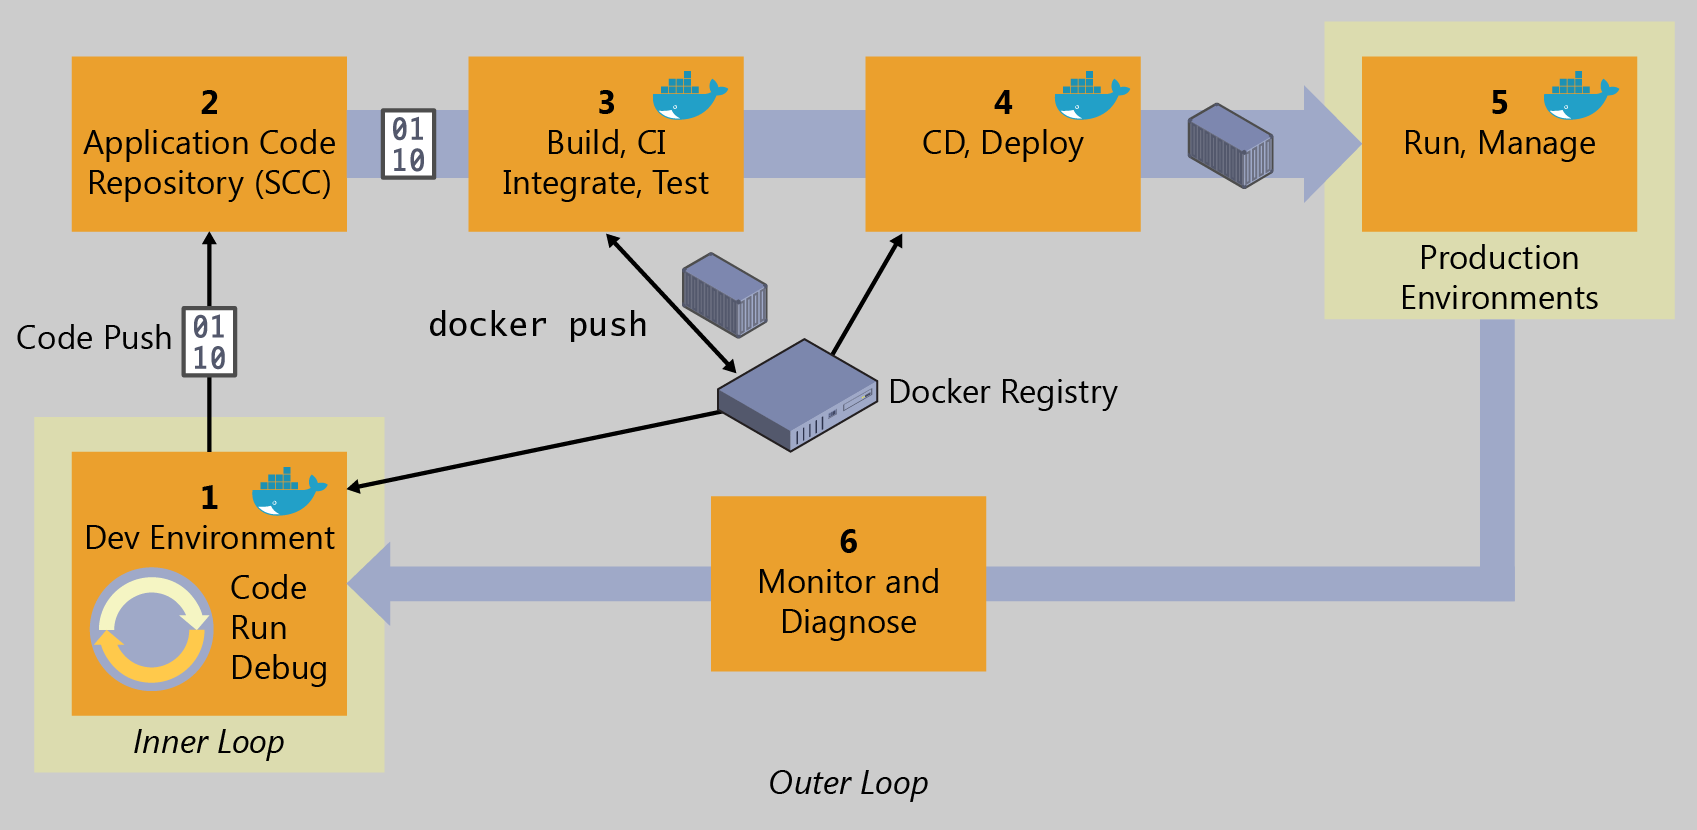
\includegraphics[width=10cm]{img/docker_process.png}
\end{frame}